\documentclass[12pt]{article}
\usepackage[margin=2cm]{geometry}
\usepackage{amsmath}
\usepackage{graphicx}
\usepackage{enumitem}
\graphicspath{ {./} }

\title{IT'S LIKE A TEST}
\author{School Year 2022/2023}
\date{
  Primary\endgraf
  Study Field: Mathematics 
}

\begin{document}
\maketitle
\newpage

\begin{center}
  \title{\textbf{\Large Test something something}\\[1ex]
    \textbf{\LARGE By Kureji Ollie}\\[2ex]
    \textbf{\large Hololive ID Gen 2}}
\end{center}

\hrule

\begin{center}
  \textbf{Test something something}\\
  \vspace{0.5cm}

  \begin{tabular}{l @{\hspace{1cm}} l}
    \text{Subject} & : Mathematics                 \\
    \text{Event}   & : They say Zeta pen streaming \\
    \text{Date}    & : Sunday, 29 April 2023       \\
    \text{Time}    & : Until things are done       \\
  \end{tabular}
\end{center}

\textbf{Instructions:} \\
\text{1. There are 10 essay questions.}\\
\text{2. Do the questions that you find easy first.}\\
\text{3. If you can't, wave at the camera while shouting "OLLIE-SENPAI BOING BOINGNYA TOP} \\
\text{TOP MARKOTOP WANJAY"}
\vspace{0.5cm}
\hrule

\vspace{0.5cm}

\begin{enumerate}
  \item $(8x-12)(6x+7)$\\
        \\
        The product of the above algebra is\ldots\\
        (Algebra, Grade 7)\\


  \item One day, Kiko decided to ride a bike around the complex. During the ride, the wheel rotates $220$ times, resulting in the total circumference of the wheel after going around the compound being $48400$ cm. Find the area of Kiko's bicycle wheel so that Kiko can sleep tonight!\\
        (2D Geometry, Grade 8)

  \item Find $r$ in the given shape (3D Geometry, Grade 9) \\
        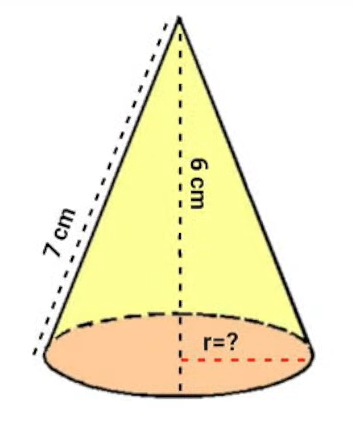
\includegraphics{3-shape.png}

        \begin{center}
          \title{\textbf{\Large Test something something}\\[1ex]
            \textbf{\LARGE By Kureji Ollie}\\[2ex]
            \textbf{\large Hololive ID Gen 2}}
        \end{center}
        \hrule

  \item If $log_2 \, 3 = x$, then the value of $log_8 \, 12$ is\ldots\\
        (Logarithm, Grade 10)

  \item $f(x) = 4x^2 + 3x + 8$ [$A$] \\
        $g(x) = ax^2 + bx + c$ [$B$] \\
        Function $A$ has the same form as function $B$. Calculate $9a+8b+7c$. \\
        (Quadratic Function, Grade 10)

  \item In 2019, a steam wallet filling service is doing business.

        The cheapest wallet filling is IDR $45\,000$, and he offers IDR $50\,000$ for each filling. Meanwhile, the most expensive wallet filling is IDR $900\,000$, and he offers IDR $905\,000$ for each filling.

        The capital he prepared was IDR $5\,500\,000$ for doing business. If $x$ represents the number of fillings for the cheapest wallet and $y$ represents the most expensive wallet filling, then the most appropriate target function for the fish trader to get the maximum profit is\ldots \\
        (Target Function, Grade 11)

  \item Given an arithmetic sequence 2, 5, 8, \ldots, $u_n = 144$. Determine the number of terms ($n$)! \\
        (Arithmetic Sequence, Grade 11)

  \item In a free gacha event, there is Box 1 containing $2$ Oshi A stickers and $4$ Oshi B stickers. Meanwhile, Box 2 contains $5$ Oshi A stickers and $3$ Oshi B stickers. 1 sticker is taken from each box. The probability of getting an Oshi A sticker from Box 1 and an Oshi B sticker from Box 2 is... \\
        (Probability, Grade 12)

  \item The $2^{nd}$ and $5^{th}$ terms of a geometric sequence are $1$ and $8$, respectively. Find the value of the $11^{th}$ term! \\
        (Geometric Sequence, Grade 12)

  \item Find the (first) derivative of the functions below:
        \begin{enumerate}[label=\alph*)]
          \item $f(x) = 8 \sqrt{x}$
          \item $f(x) = \frac{x}{2} $
          \item $f(x) = x^2 + 4$
        \end{enumerate}
        (Derivative Function, Grade 12)
\end{enumerate}

\end{document}
